%%%%%%%%%%%%%%%%%%%%%%%%%%%%%%%%%%%%%%%%%
% Short Sectioned Assignment LaTeX Template Version 1.0 (5/5/12)
% This template has been downloaded from: http://www.LaTeXTemplates.com
% Original author:  Frits Wenneker (http://www.howtotex.com)
% License: CC BY-NC-SA 3.0 (http://creativecommons.org/licenses/by-nc-sa/3.0/)
%%%%%%%%%%%%%%%%%%%%%%%%%%%%%%%%%%%%%%%%%

%----------------------------------------------------------------------------------------
%	PACKAGES AND OTHER DOCUMENT CONFIGURATIONS
%----------------------------------------------------------------------------------------

\documentclass[paper=a4, fontsize=10pt]{article} % A4 paper and 11pt font size

% ---- Entrada y salida de texto -----

\usepackage[T1]{fontenc} % Use 8-bit encoding that has 256 glyphs
\usepackage[utf8]{inputenc}
%\usepackage{fourier} % Use the Adobe Utopia font for the document - comment this line to return to the LaTeX default

% ---- Idioma --------

\usepackage[spanish, es-tabla]{babel} % Selecciona el español para palabras introducidas automáticamente, p.ej. "septiembre" en la fecha y especifica que se use la palabra Tabla en vez de Cuadro

% ---- Otros paquetes ----

\usepackage{amsmath,amsfonts,amsthm} % Math packages
%\usepackage{graphics,graphicx, floatrow} %para incluir imágenes y notas en las imágenes
\usepackage{graphics,graphicx, float, url} %para incluir imágenes y colocarlas

% Para hacer tablas comlejas
%\usepackage{multirow}
%\usepackage{threeparttable}

%\usepackage{sectsty} % Allows customizing section commands
%\allsectionsfont{\centering \normalfont\scshape} % Make all sections centered, the default font and small caps

\usepackage{fancyhdr} % Custom headers and footers
\pagestyle{fancyplain} % Makes all pages in the document conform to the custom headers and footers
\fancyhead{} % No page header - if you want one, create it in the same way as the footers below
\fancyfoot[L]{} % Empty left footer
\fancyfoot[C]{} % Empty center footer
\fancyfoot[R]{\thepage} % Page numbering for right footer
\renewcommand{\headrulewidth}{0pt} % Remove header underlines
\renewcommand{\footrulewidth}{0pt} % Remove footer underlines
\setlength{\headheight}{13.6pt} % Customize the height of the header

\numberwithin{equation}{section} % Number equations within sections (i.e. 1.1, 1.2, 2.1, 2.2 instead of 1, 2, 3, 4)
\numberwithin{figure}{section} % Number figures within sections (i.e. 1.1, 1.2, 2.1, 2.2 instead of 1, 2, 3, 4)
\numberwithin{table}{section} % Number tables within sections (i.e. 1.1, 1.2, 2.1, 2.2 instead of 1, 2, 3, 4)

\setlength\parindent{0pt} % Removes all indentation from paragraphs - comment this line for an assignment with lots of text

\newcommand{\horrule}[1]{\rule{\linewidth}{#1}} % Create horizontal rule command with 1 argument of height

\usepackage{url} %bibliografía
\usepackage{appendix}
\usepackage{sectsty}
\usepackage{listings}
\usepackage{xcolor}
\usepackage{colortbl}
\usepackage{breakurl}
%\usepackage{hyperref}
%\usepackage[breaklinks=true]{hyperref}
\usepackage[hidelinks]{hyperref} 
\usepackage{fancyvrb}
\usepackage{color}

\usepackage{multirow} % para las tablas


\usepackage{anysize}
\marginsize{3cm}{3cm}{2.5cm}{2.5cm} %izq, derecha, arriba
% Se limpia la cabecera y el pie de página para poder rehacerlos luego.

% Espacios en el documento:
\linespread{1}                        % Espacio entre líneas.
\setlength\parindent{0pt}               % Selecciona la indentación para cada inicio de párrafo.


\lstset{
        tabsize=2, % tab = 2 espacios
        backgroundcolor=\color[HTML]{F0F0F0}, % color de fondo
        captionpos=b, % posición de pie de código, b=debajo
        basicstyle=\ttfamily, % estilo de letra general
        columns=fixed, % columnas alineadas
        extendedchars=true, % ASCII extendido
        breaklines=true, % partir líneas
        %prebreak = \raisebox{0ex}[0ex][0ex]{\ensuremath{\hookleftarrow}}, % marcar final de línea con flecha
        showtabs=false, % no marcar tabulación
        showspaces=false, % no marcar espacios
        keywordstyle=\bfseries\color[HTML]{007020}, % estilo de palabras clave
        commentstyle=\itshape\color[HTML]{60A0B0}, % estilo de comentarios
        stringstyle=\color[HTML]{4070A0}, % estilo de strings
}

\renewcommand{\appendixname}{Anexos}
\renewcommand{\appendixtocname}{Anexos}
\renewcommand{\appendixpagename}{Anexos}

\title{	
\normalfont \normalsize 
\textsc{{\bf Sistemas multimedia (2018-2019)} \\ Grado en Ingeniería Informática \\ Universidad de Granada} \\ [25pt] % Your university, school and/or dbrewepartment name(s)
\horrule{0.5pt} \\[0.4cm] % Thin top horizontal rule
\huge Domentación Paint. Práctica de Evaluación. \\ % The assignment title
\horrule{2pt} \\[0.5cm] % Thick bottom horizontal rule
}
\author{Montserrat Rodríguez Zamorano} % Nombre y apellidos
\date{\normalsize\today} % Incluye la fecha actual

\begin{document}
\pagestyle{empty}
\maketitle
\vskip1cm
\clearpage
\tableofcontents
\clearpage
%\vskip0.3cm
%\begin{figure}[H]
 % \centering
  %  \includegraphics[width=0.8\textwidth]{}
 % \caption{Diseño conceptual}
 % \label{diseño}
%\end{figure}
\setcounter{page}{1}
\pagestyle{plain}
\section{Descripción del sistema}
Para la evaluación de la asignatura de \textit{Sistemas multimedia} se quiere realizar una aplicación multimedia que permita gestionar gráficos, imágenes, sonido y vídeo. Se podrá crear, editar, procesar y visualizar contenido multimedia de distintos tipos.
\vskip0.3cm
Esta aplicación tendrá una ventana principal con diferentes barras de herramientas y botones que permitirán realizar las distintas operaciones sobre el contenido multimedia. Se intentará que la interfaz sea lo más intuitiva posible y facilitar así el uso de la aplicación al usuario final.
\vskip0.3cm
Con este fin, se realiza una aplicación que se llamará \textit{Paint}.
\section{Requisitos}
\subsection{Requisitos funcionales}
\subsubsection{Carácter general}
\begin{itemize}
\item{\textbf{[RFCG-1]} Creación de una nueva imagen en una nueva ventana.}
\item{\textbf{[RFCG-2} Abrir un fichero de imagen.}
\item{\textbf{[RFCG-3]} Abrir un fichero de sonido.}
\item{\textbf{[RFCG-4]} Abrir un fichero de vídeo.}
\item{\textbf{[RFCG-5]} Guardar una imagen y sus figuras dibujadas.}
\item{\textbf{[RFCG-6]} Ocultar las barras de herramientas.}
\item{\textbf{[RFCG-7]} Visualizar las barras de herramientas.}
\item{\textbf{[RFCG-8]} Consultar el nombre del programa, versión y autor.}
\end{itemize}
\subsubsection{Dibujo}
\begin{itemize}
\item{\textbf{[RFD-1]} Dibujar las siguientes formas geométricas con sus propios atributos independientes.
\begin{itemize}
\item{Línea.}
\item{Rectángulo.}
\item{Elipse.}
\item{Rectángulo con esquinas redondeadas.}
\end{itemize}
}
\item{\textbf{[RFD-2]} Mantener todas las figuras que se vayan dibujando.}
\item{\textbf{[RFD-3]} Elegir el color de trazo de dibujo.
\begin{itemize}
\item{Rojo.}
\item{Azul.}
\item{Negro.}
\item{Blanco.}
\item{Verde.}
\end{itemize}
}
\item{\textbf{[RFD-4]} No rellenar la imagen.}
\item{\textbf{[RFD-5]} Rellenar con color el dibujo.
\begin{itemize}
\item{Rojo.}
\item{Azul.}
\item{Negro.}
\item{Blanco.}
\item{Verde.}
\end{itemize}
}
\item{\textbf{[RFD-6]} Seleccionar una figura dibujada.}
\item{\textbf{[RFD-7]} Editar una figura dibujada.}
\item{\textbf{[RFD-8]} Mover una figura dibujada.}
\item{\textbf{[RFD-9]} Consultar los atributos de una figura dibujada.}
\item{\textbf{[RFD-10]} Asociar un grado de transparencia a una figura.}
\item{\textbf{[RFD-11]} Activar alisado de bordes de una figura.}
\item{\textbf{[RFD-12]} Desactivar alisado de bordes de una figura.}
\end{itemize}
\subsubsection{Procesamiento de imágenes}
\begin{itemize}
\item{\textbf{[RFPI-1]} Duplicar una imagen.}
\item{\textbf{[RFPI-2]} Modificar el brillo de una imagen.}
\item{\textbf{[RFPI-3]} Aplicar filtro para emborronar una imagen.}
\item{\textbf{[RFPI-4]} Aplicar filtro para enfocar una imagen.}
\item{\textbf{[RFPI-5]} Aplicar filtro de relieve a una imagen.}
\item{\textbf{[RFPI-6]} Aplicar contraste a una imagen.}
\item{\textbf{[RFPI-7]} Iluminar una imagen.}
\item{\textbf{[RFPI-8]} Oscurecer una imagen.}
\item{\textbf{[RFPI-9]} Extraer las bandas de una imagen.}
\item{\textbf{[RFPI-10]} Invertir los colores de una imagen.}
\item{\textbf{[RFPI-11]} Convertir una imagen a los siguientes espacios:
\begin{itemize}
\item{RGB}
\item{YCC}
\item{GRAY}
\end{itemize}
}
\item{\textbf{[RFPI-12]} Girar una imagen a cualquier ángulo.}
\item{\textbf{[RFPI-13]} Tintar una imagen.}
\item{\textbf{[RFPI-14]} Escoger nivel de tintado de una imagen.}
\item{\textbf{[RFPI-15]} Ecualizar una imagen.}
\item{\textbf{[RFPI-16]} Umbralizar una imagen en niveles de gris.}
\item{\textbf{[RFPI-17]} Escoger nivel de umbralización.}
\item{\textbf{[RFPI-18]} Aplicar filtro sepia a una imagen.}
\item{\textbf{[RFPI-19]} Aplicar filtro violeta a una imagen.}
\item{\textbf{[RFPI-20]} Aplicar filtro de media entre las bandas de colores.}
\item{\textbf{[RFPI-21]} Aplicar filtro cosinosuidal.}
\end{itemize}
\subsubsection{Sonido}
\begin{itemize}
\item{\textbf{[RFS-1]} Reproducir audios.}
\item{\textbf{[RFS-2]} Grabar sonidos.}
\item{\textbf{[RFS-3]} Pausar la reproducción.}
\item{\textbf{[RFS-4]} Parar la grabación.}
\item{\textbf{[RFS-5]} Parar la reproducción.}
\end{itemize}
\subsubsection{Vídeo}
\begin{itemize}
\item{\textbf{[RFV-1]} Mostrar la secuencia que capte la Webcam.}
\item{\textbf{[RFV-2]} Capturar una imagen desde la Webcam.}
\end{itemize}
\subsection{Requisitos no funcionales}
\begin{itemize}
\item{\textbf{[RNF-1]} Se mostrará en la barra de estado el pixel en el que está situado el ratón.}
\item{\textbf{[RNF-2]} Se habilitarán en cada momento sólo los botones que pueden utilizarse. Por ejemplo, si se abre una ventana de vídeo se deshabilitarán aquellos correspondientes a las imágenes.}
\item{\textbf{[RNF-3]} Los botones tendrán asociados un \textit{ToolTipText} para facilitar el uso del programa.}
\item{\textbf{[RNF-4]} Al seleccionar una figura se activarán sus propiedades en la barra de atributos.}
\item{\textbf{[RNF-5]} Si hay una figura seleccionada, al pulsar el ratón sobre en otro punto, deberá deseleccionarse la figura.}
\item{\textbf{[RNF-6]} El título de una nueva ventana abierta será el nombre del fichero si se trata de una imagen abierta o guardada.}
\item{\textbf{[RNF-7]} El título de una nueva ventana abierta será \textit{Nueva} si se trata de una imagen creada por el usuario.}
\item{\textbf{[RNF-8]} El título de una nueva ventana abierta será \textit{Captura} si se trata de una captura captada de un vídeo o de la WebCam.}
\item{\textbf{[RNF-9]} La \textit{BoundingBox} será un rectángulo de color azul, con línea discontinua.}
\item{\textbf{[RNF-10]} Cuando se cree una imagen se lanzará un diálogo que permita elegir las dimensiones de la imagen.}

\end{itemize}

\clearpage

\section{Análisis}
Se hará un análisis del problema y de las posibles soluciones, intentando que sea lo más independiente posible del lenguaje de programación. En el apartado de \textit{Diseño} se especificarán detalles relacionados con la programación.
\vskip0.3cm
En primer lugar, se plantea cómo debería ser el área de dibujo, que almacenará los atributos con los que se pintará la siguiente figura. Con este fin se desarrollará una clase \textit{Lienzo}. Esta clase será la encargada de pintar las figuras. Cada figura dibujada en el área de dibujo tendrá los atributos activos en ese momento en el lienzo, si bien sus atributos podrán modificarse a posteriori.
\vskip0.3cm
La solución planteada durante el desarrollo de las prácticas no es muy flexible: la biblioteca \texttt{java.awt.Graphics} ofrece importantes limitaciones, ya que no permite que los objetos tengan propiedades de color, forma o grosor, entre otras. De esta forma, todas las figuras de un mismo lienzo se pintarán con los mismos atributos.
\vskip0.3cm
Para que cada figura tenga sus propios atributos se desarrollará una clase propia \textit{Figura}, que almacenará cada uno de los atributos de la figura y permitirá que cada figura tenga los suyos propios: color, grosor, etc. Sin embargo, la línea, por ejemplo, no puede tener relleno, por lo que no tiene sentido guardar este atributo. Se desarrollará una clase propia para cada una de las figuras que pueden dibujarse: Línea, rectángulo, elipse, rectángulo redondeado.
\vskip0.3cm
Para intentar mejorar el diseño de esta clase, en lugar de que las formas hereden directamente de \textit{Figura}, se dividirán en dos grupos: figuras rellenables y figuras lineales. De esta forma, las operaciones comunes relativas al relleno podrán realizarse en el ámbito de la figura rellenable, y no tener que implementarlas en cada una de las clases derivadas. Con esta jerarquía de clases, evitamos que figuras lineales tengan atributos que no deben tener, como por ejemplo, tipo de relleno, así como evitamos que en figuras con propiedades similares (elipse y rectángulo, por ejemplo) se repitan funciones o atributos.
\vskip0.3cm
\begin{figure}[H]
 \centering
  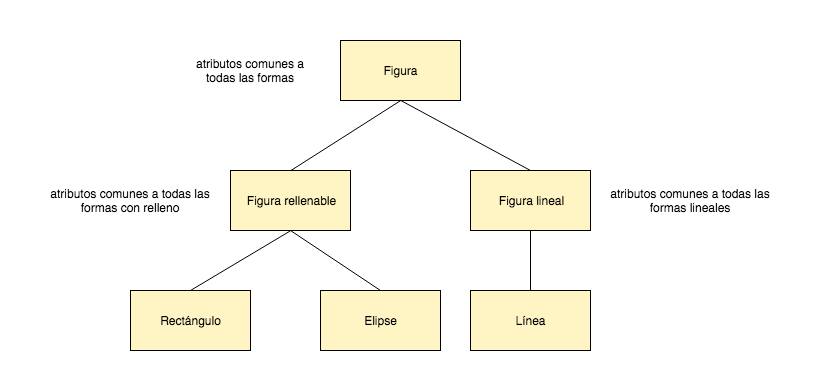
\includegraphics[width=0.8\textwidth]{esquemaFormas.png}
 \caption{Esquema del diseño de la clase \textit{Figura}}
 \label{diseño}
 \end{figure}
\vskip0.3cm
Uno de los métodos que tendrá que implementar en cada clase por separado será \textit{setLocation}. En principio se pretendía aprovechar el método que proporcionaba \texttt{Graphics}, pero se ha optado por implementarlo en cada clase de forma manual, ya que para \texttt{Rectangle2D} y \texttt{Ellipse2D} no está disponible el uso de esta función.
\vskip0.3cm
En cuanto al manejo de eventos, se usará en muchas ocasiones las funciones que ofrece Java para la gestión de eventos (por ejemplo, para el uso de botones en la ventana principal). Sin embargo, para la comunicación entre el lienzo y la ventana principal será necesario crear una clase manejadora para la gestión de eventos relacionados con el lienzo. La existencia de esta clase permitirá por ejemplo informar de la falta de atributos necesarios para el dibujo de las figuras y poder lanzar mensajes de error desde la ventana principal (por ejemplo: no se ha seleccionado una forma de dibujo) o informar a la ventana principal de la creación de una nueva figura, para que aparezca en una lista desplegable de figuras seleccionables. 
%%%%%%%%%%%%%%%%%%% DISEÑO %%%%%%%%%%%%%%%%
\clearpage
\section{Diseño}
Siguiendo la propuesta que se ha planteado en el análisis, se plantea las siguientes jerarquías de clases. Mientras la propuesta anterior intentaba ser independiente del lenguaje de programación, en este apartado se especifican aspectos concretos de la implementación en \textit{Java}.
\vskip0.3cm
Se hará una descripción general, pero para más detalles se pueden consultar los diagramas de clase.
\subsection{VentanaPrincipal}
La clase \texttt{VentanaPrincipal} implementará la visión principal del programa. Heredará de \texttt{JFrame} y contendrá múltiples elementos \texttt{Swing}:
\begin{itemize}
\item{\textbf{Barras de herramientas:} serán del tipo \texttt{JToolBar}, y se tratan de las barras superior, izquierda y derecha. Serán las que contendrán la mayoría de los demás elementos \texttt{Swing}.}
\item{\textbf{Barra de estado:} se trata de un elemento \texttt{JPanel} que contendrá elementos del tipo \texttt{JLabel}. El texto de estas etiquetas indicarán, por ejemplo, que una figura ha sido añadida.}
\item{\textbf{Listas desplegables:} se utilizarán \texttt{JComboBox}.}
\item{\textbf{Botones \texttt{JToggleButton}:} pueden quedarse seleccionados, por lo que se utilizarán para las formas, o para los botones de sonido, pudiendo agruparse en distintos grupos \texttt{ButtonGroup}.}
\item{\textbf{Botones \texttt{JButton}:} En el caso de por ejemplo, los filtros, no tiene demasiado interés que un botón quede seleccionado, por lo que para la mayoría de las operaciones de procesamiento de imágenes se utilizará este tipo de botones.}
\item{\textbf{Escritorio:} se trata de un elemento del tipo \texttt{JDesktopPane}. Este escritorio será aquel que contendrá las ventanas multimedia de distintos tipos.}
\end{itemize}

\subsection{Lienzo}

\subsection{Ventanas internas}
Se definirá una clase \texttt{VentanaMultimedia} que heredará \texttt{JInternalFrame}. De esta clase derivarán diferentes ventanas en función del archivo multimedia que contengan.
\begin{itemize}
\item{\textbf{VentanaMultimediaImagen:} se encargará de almacenar el contenido multimedia de tipo imagen. Tendrá un objeto de clase \texttt{LienzoImagen}, que será un rectángulo en blanco en el caso de que sea creada por el usuario, y una imagen en el caso de que sea una imagen abierta. Contendrá también un elemento de tipo 	\texttt{JScrollPane} para el caso en que la ventana no pueda contener la imagen completa.}
\item{\textbf{VentanaMultimediaCamara:} se encargará de almacenar las imágenes que pueden verse desde la WebCam así como las funciones encargadas de gestionar este contenido.}
\item{\textbf{VentanaMultimediaVLCPlayer:} se encargará de almacenar vídeos así como las funciones encargadas de gestionar este contenido.}
\end{itemize}
\subsection{Figura}
Se definirá una clase abstracta \texttt{Figura}. Esta clase almacenará los atributos de la figura. Las clases \texttt{FiguraRellenable} y \texttt{FiguraLineal} heredarán de \texttt{Figura}. Aunque en este caso no hay más de una figura lineal, este esquema permite que en posteriores versiones se añadan curvas u otro tipo de figuras lineales. De \texttt{FiguraRellenable} heredarán \texttt{Rectangulo},\texttt{Elipse} y \texttt{RectanguloRedondeado}. De \texttt{FiguraLineal} heredará la clase \texttt{Linea}. Cada una de estas clases tendrá asociado un objeto \texttt{Shape}, además de los atributos de las clases de las que hereda.\vskip0.3cm
Es esta jerarquía de clases la que permite que cada figura tenga sus propios atributos, así como la posibilidad de cambiarlos.
\subsection{Gestión de eventos}
Se hará uso de las funciones de gestión de eventos que ofrece \textit{Java}. Sin embargo, es necesario implementar las funciones para la gestión de eventos en el lienzo, de forma que podamos establecer una comunicación entre lienzo y ventana principal.
\begin{itemize}
\item{\textbf{LienzoEvent:}}
\item{\textbf{LienzoListener:}}
\item{\textbf{LienzoAdapter:}}
\item{\textbf{MiManejadorLienzo:}}
\end{itemize}
\subsection{Procesamiento de imágenes}
\subsubsection{Operador \textit{LookUpOp}}

\subsubsection{Componente a componente}
La función componente a componente modificará cada una de las componentes (R, G, B) de forma separada.\vskip0.3cm
En este caso se ha implementado un filtro violeta. Para aplicar un tono morado a la imagen, se tendrá en cuenta que la mezcla de rojo y azul es la que da lugar al morado. Por tanto, para obtener el efecto deseado se reducirá el valor de la componente verde y se aumentará el valor de la componente roja y azul.
\vskip0.3cm
Además, como se ha aumentado el valor de las componentes de forma significativa, habrá un aumento de la luminosidad en estos colores y de la intensidad de la imagen en general.
\begin{lstlisting}[language=Java, caption=Operación componente a componente, label=lst:graddesc]
for(int x=0; x<src.getWidth(); x++){
    for(int y=0; y<src.getHeight(); y++){
        int destR, destG, destB;
        int srcR, srcG, srcB;
        Color colorSrc = new Color(src.getRGB(x, y));
        Color colorDest;
        //color del pixel
        srcR = colorSrc.getRed();
        srcG = colorSrc.getGreen();
        srcB = colorSrc.getBlue();
        //operacion componente a componente
        destR = (int) Math.min(255,1.3*srcR);
        destG = (int) Math.min(255,0.2*srcG);
        destB = (int) Math.min(255,1.5*srcB);
                
        colorDest = new Color(destR, destG, destB);
        dest.setRGB(x, y, colorDest.getRGB());
     }
}
\end{lstlisting}
El resultado de aplicar el filtro puede verse a continuación. Como se puede ver, se obtiene el resultado deseado.
\vskip0.3cm
\begin{figure}[H]
 \centering
  
\includegraphics[width=0.3\textwidth]{imagenes/Fry.jpg}
  
\includegraphics[width=0.3\textwidth]{imagenes/fryVioleta.jpg}
 \caption{Aplicación filtro violeta sobre \texttt{Fry.jpg}}
 \label{diseño}
 \end{figure}

\vskip0.3cm
\begin{figure}[H]
 \centering
  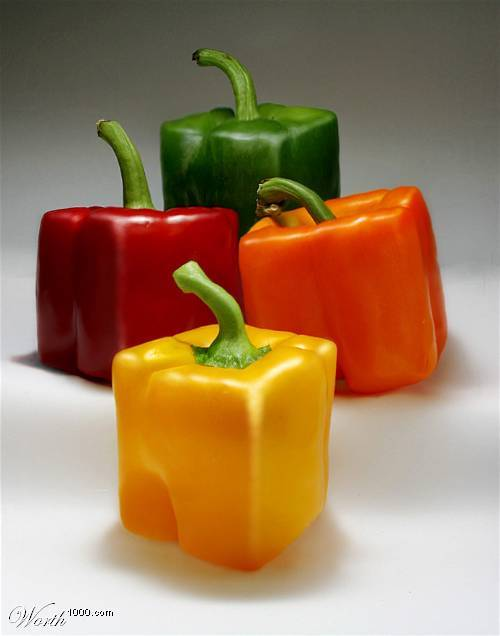
\includegraphics[width=0.3\textwidth]{imagenes/pimientos.jpg}
  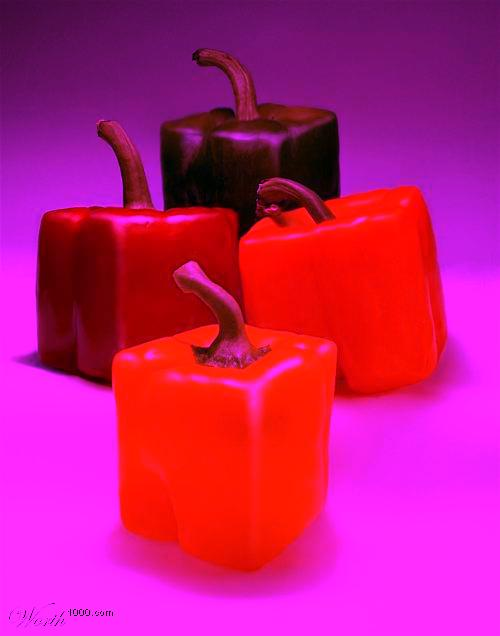
\includegraphics[width=0.3\textwidth]{imagenes/pimientosVioleta.jpg}
 \caption{Aplicación filtro violeta}
 \label{diseño}
 \end{figure} 
 
\subsubsection{Primera operación píxel a píxel}
La función píxel a píxel modificará cada componente teniendo en cuenta los demás componentes, de forma que el valor de cada componente podrá ser una combinación de las otras.
\vskip0.3cm
La operación implementada en este caso es una especie de "filtro rojizo", aunque no llega a serlo como tal. El valor del color rojo se conservará tal y como está, mientras que los valores verde y azul serán una media de los otros tres, por lo que aquellos píxeles en los que estos valores sean predominantes tendrán un color grisáceao.
\vskip0.3cm
Se espera que en la primera aplicación del filtro, la imagen tomará este color rojizo-anaranjado, pues habrá sido la única componente que habrá mantenido su valor. Sin embargo, al estar esta componente presente en la media que asigna los valores verde y azul, a través de las sucesivas aplicaciones del filtro estos dos valores convergerán al valor de la componente roja, convirtiéndose en un filtro blanco y negro.
\begin{lstlisting}[language=Java, caption=Operación pixel a pixel, label=lst:graddesc]
for(int x=0; x<src.getWidth(); x++){
    for(int y=0; y<src.getHeight(); y++){
        int destR, destG, destB;
        int srcR, srcG, srcB;
        Color colorSrc = new Color(src.getRGB(x, y));
        Color colorDest;
        //color del pixel
        srcR = colorSrc.getRed();
        srcG = colorSrc.getGreen();
        srcB = colorSrc.getBlue();
        //operacion pixel a pixel
        destR = srcR;
        destG = Math.min(255,(srcR+srcG+srcB)/3);
        destB = Math.min(255,(srcR+srcG+srcB)/3);
                
        colorDest = new Color(destR, destG, destB);
        dest.setRGB(x, y, colorDest.getRGB());
    }
}
\end{lstlisting}
\vskip0.3cm
\begin{figure}[H]
 \centering
 
\includegraphics[width=0.3\textwidth]{imagenes/Fry.jpg}
  
\includegraphics[width=0.3\textwidth]{imagenes/fryMedia1.jpg}
  \vskip0.1cm
  
\includegraphics[width=0.3\textwidth]{imagenes/fryMedia2.jpg}
  
\includegraphics[width=0.3\textwidth]{imagenes/fryMedia3.jpg}
 \caption{Aplicaciones sucesivas operación píxel a píxel (I)}
 \label{diseño}
 \end{figure} 

\vskip0.3cm
\begin{figure}[H]
 \centering
 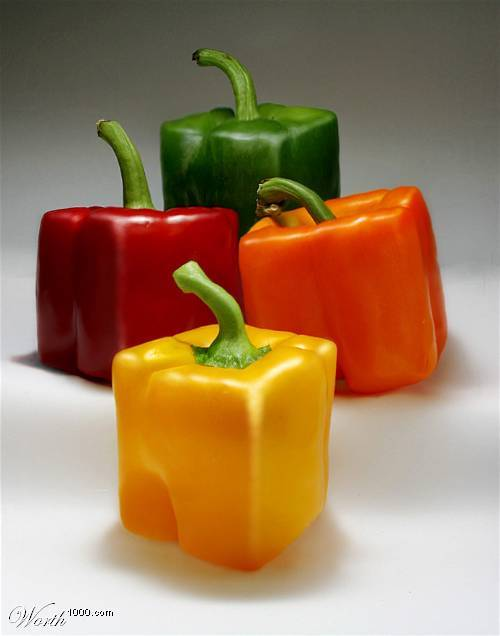
\includegraphics[width=0.3\textwidth]{imagenes/pimientos.jpg}
  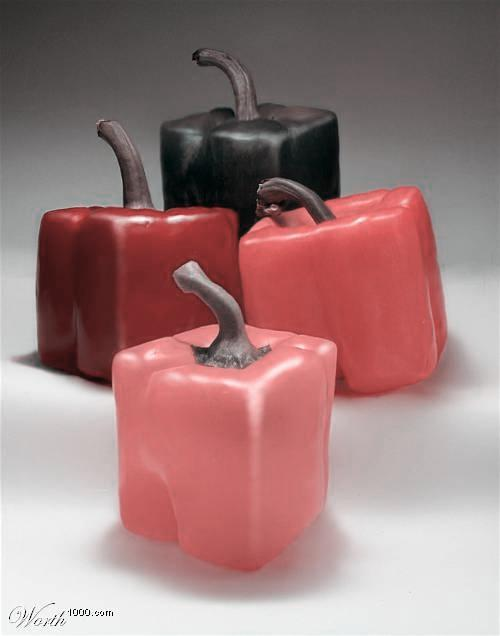
\includegraphics[width=0.3\textwidth]{imagenes/pimientosMedia1.jpg}
  \vskip0.1cm
  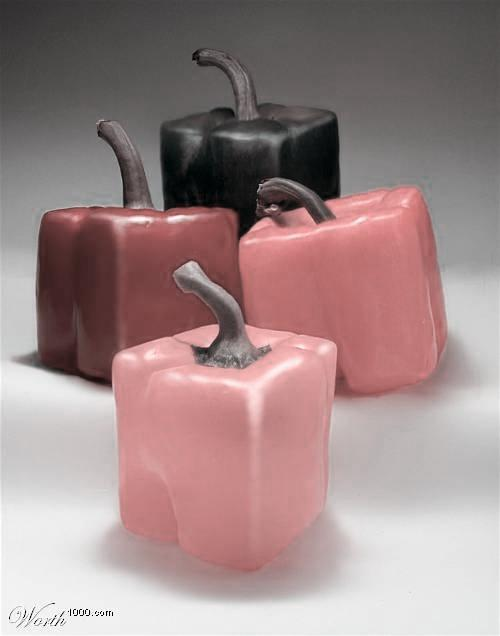
\includegraphics[width=0.3\textwidth]{imagenes/pimientosMedia2.jpg}
  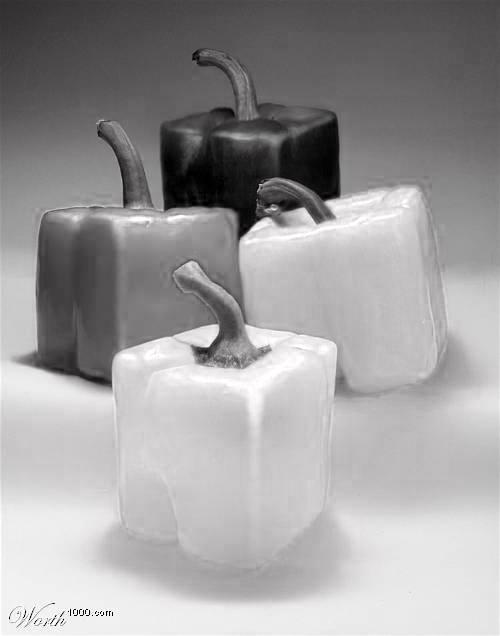
\includegraphics[width=0.3\textwidth]{imagenes/pimientosMedia3.jpg}
 \caption{Aplicaciones sucesivas operación píxel a píxel (II)}
 \label{diseño}
 \end{figure} 

\subsection{Segunda operación píxel a píxel}
Esta función es una variante de la primera, en la que se pretende que el filtro anterior no sea a través de las aplicaciones un filtro blanco y negro, sino un filtro que potencie el color rojo. Para ello, simplemente se elimina la componente roja de la media, de forma que los valores azules y verde no convergerán al valor de la componente roja.
\vskip0.3cm
\begin{lstlisting}[language=Java, caption=Operación pixel a pixel, label=lst:graddesc]
for(int x=0; x<src.getWidth(); x++){
    for(int y=0; y<src.getHeight(); y++){
        int destR, destG, destB;
        int srcR, srcG, srcB;
        Color colorSrc = new Color(src.getRGB(x, y));
        Color colorDest;
        //color del pixel
        srcR = colorSrc.getRed();
        srcG = colorSrc.getGreen();
        srcB = colorSrc.getBlue();
        //operacion pixel a pixel
        destR = srcR;
        destG = (srcG+srcB)/2;
        destB = (srcG+srcB)/2;
                
        colorDest = new Color(destR, destG, destB);
        dest.setRGB(x, y, colorDest.getRGB());
    }
}
\end{lstlisting}
A continuación pueden verse ejemplos de la aplicación de este filtro, que ofrece el resultado esperado.
\vskip0.3cm
\begin{figure}[H]
 \centering
 
\includegraphics[width=0.3\textwidth]{imagenes/Fry.jpg}
  
\includegraphics[width=0.3\textwidth]{imagenes/fryRojido.jpg}
  \vskip0.3cm
  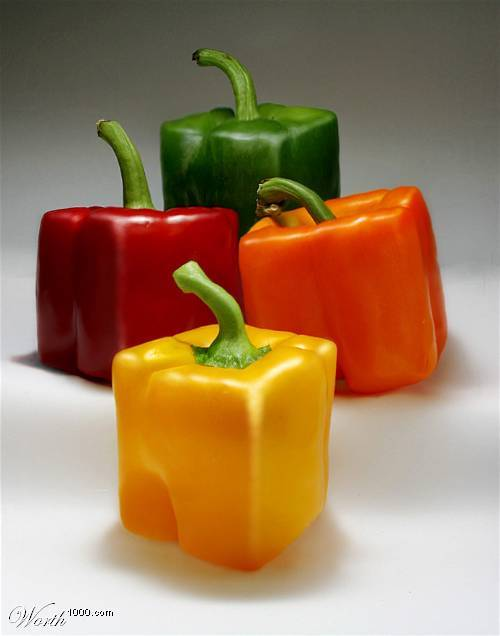
\includegraphics[width=0.3\textwidth]{imagenes/pimientos.jpg}
  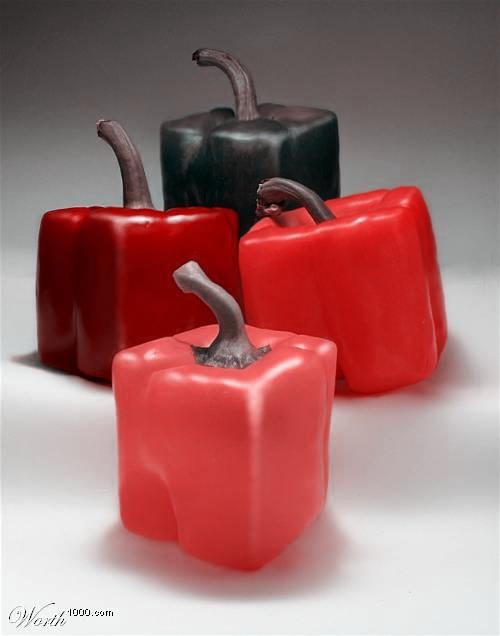
\includegraphics[width=0.3\textwidth]{imagenes/pimientoRojizo.jpg}
 \caption{Aplicación filtro rojizo}
 \label{diseño}
 \end{figure}
%%%%%%%%%%%%%%%%%%%%% IMPLEMENTACION %%%%%%%%%%%%%%%%%%%
\clearpage
\section{Implementación}
A continuación se muestra el resultado de la implementación de las clases diseñadas en el apartado anterior.
\subsection{Ventana principal}
\vskip0.3cm
\begin{figure}[H]
 \centering
  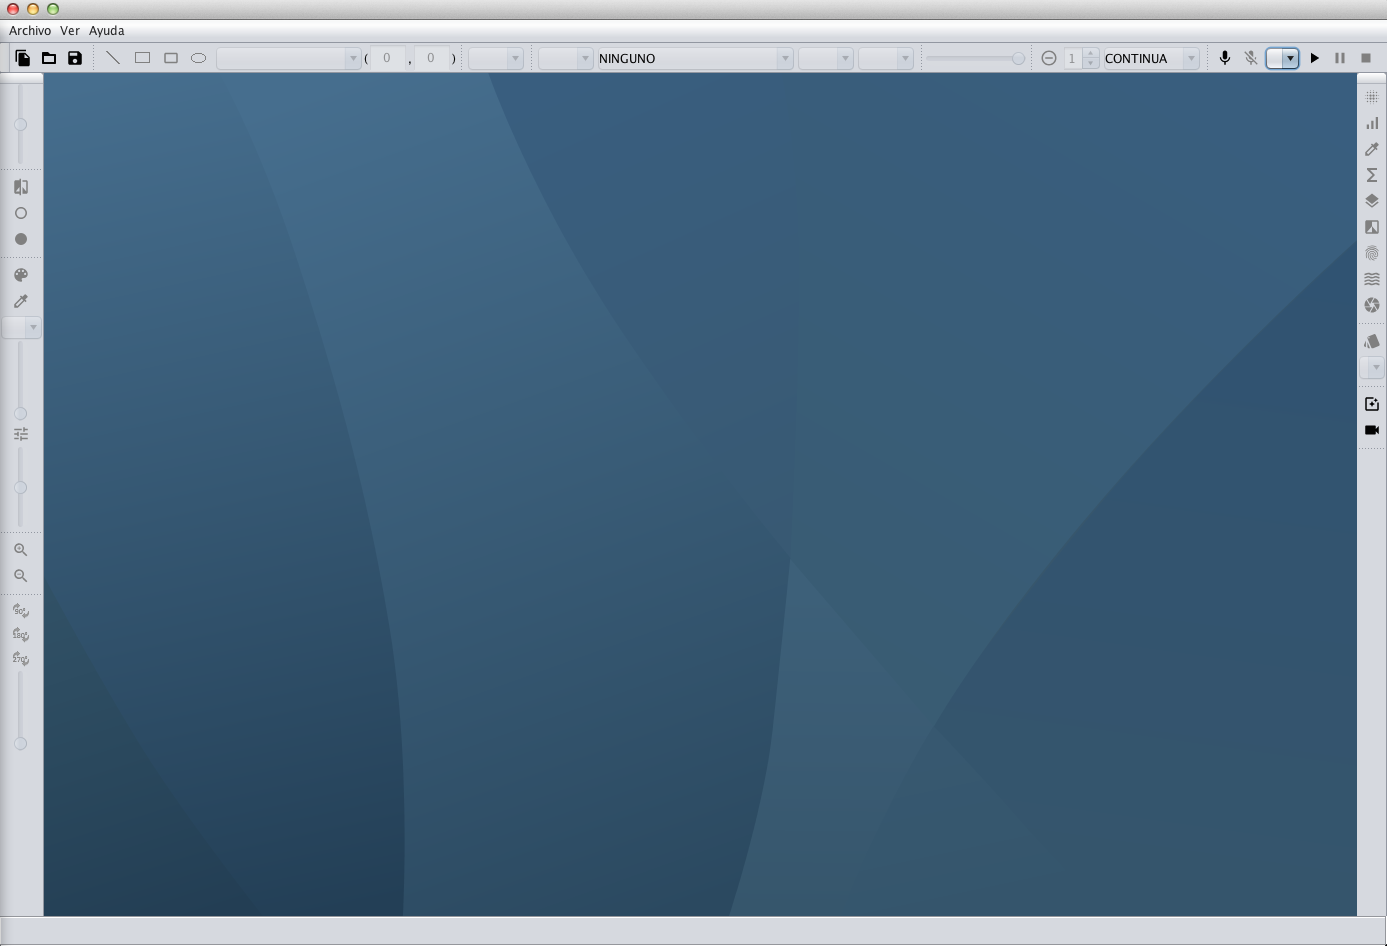
\includegraphics[width=0.8\textwidth]{graficos/ventanaPrincipal.png}
 \caption{Vista \texttt{VentanaPrincipal}}
 \label{diseño}
 \end{figure}
 
\subsection{VentanaImagen}
\vskip0.3cm
\begin{figure}[H]
 \centering
  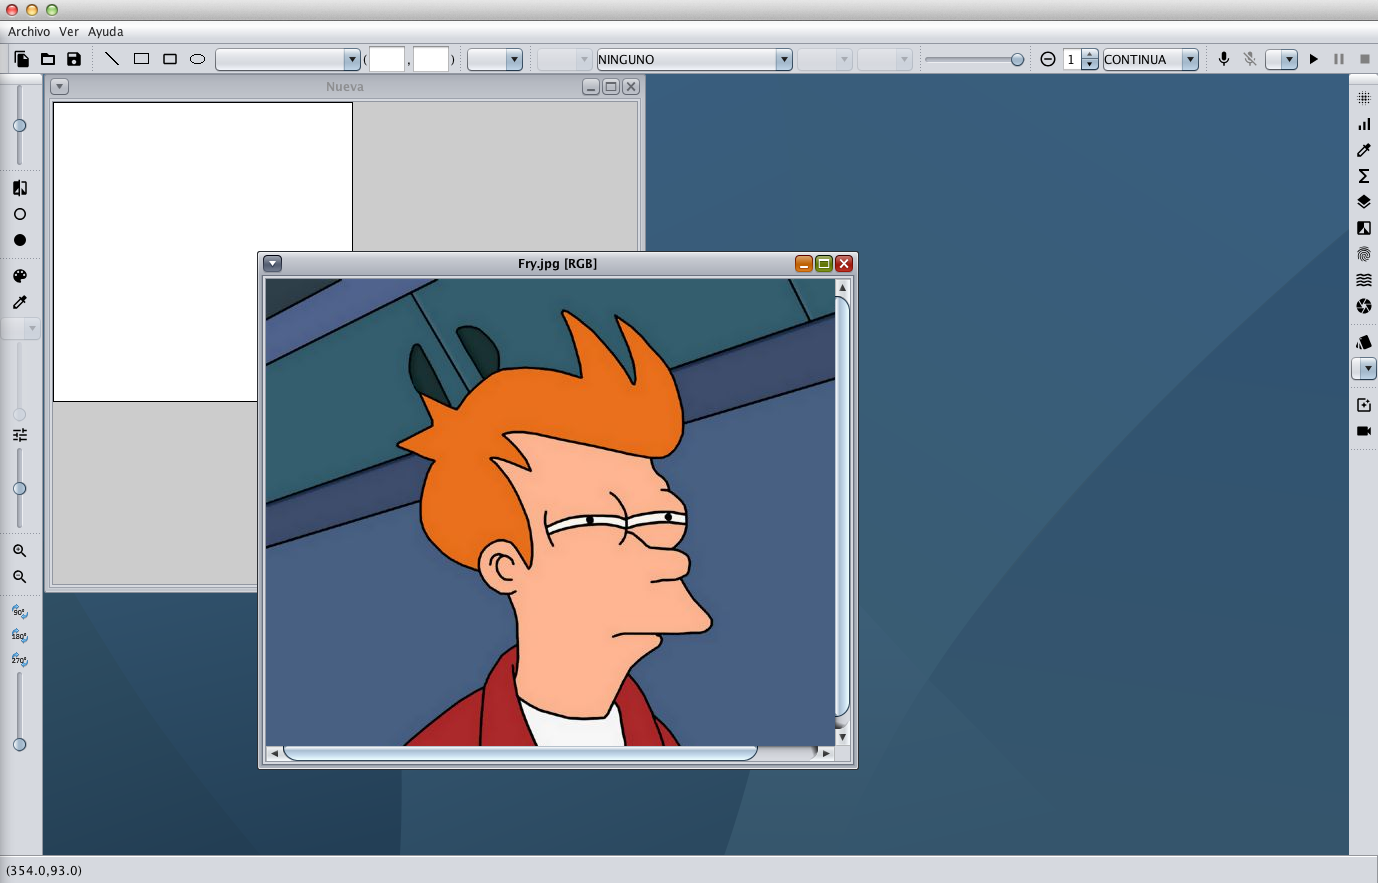
\includegraphics[width=0.7\textwidth]{graficos/ventanaImagen.jpg}
 \caption{Vista \texttt{VentanaImagen}}
 \label{diseño}
 \end{figure}
 %%%%%%%%%%%%%%%%% VALIDACION
\clearpage
\section{Validación}
En este apartado se comprobará que el programa implementado en base a la solución propuesta cumple con los requisitos enumerados en el primer apartado.
\subsection{Gráficos}
\subsection{Procesamiento de imágenes}
\subsubsection{Duplicar}
Se comprobará si la duplicación de la imagen se ha realizado correctamente, de forma que si se modifica una, los cambios no se aplican en la otra.
\vskip0.3cm
\begin{figure}[H]
 \centering
  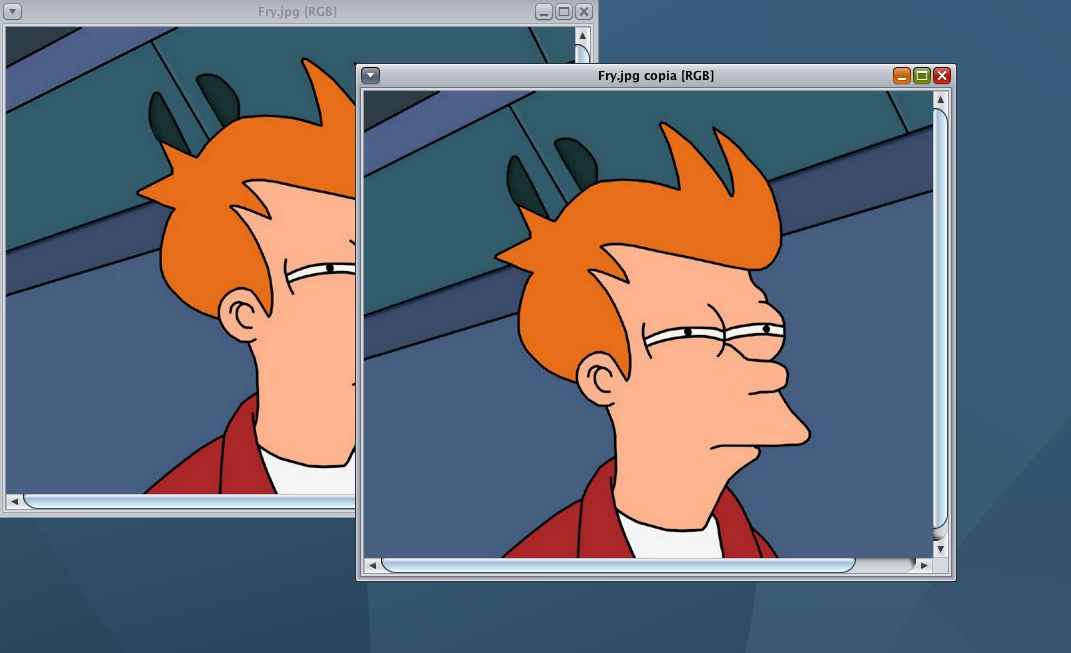
\includegraphics[width=0.5\textwidth]{imagenes/duplicar1.png}
  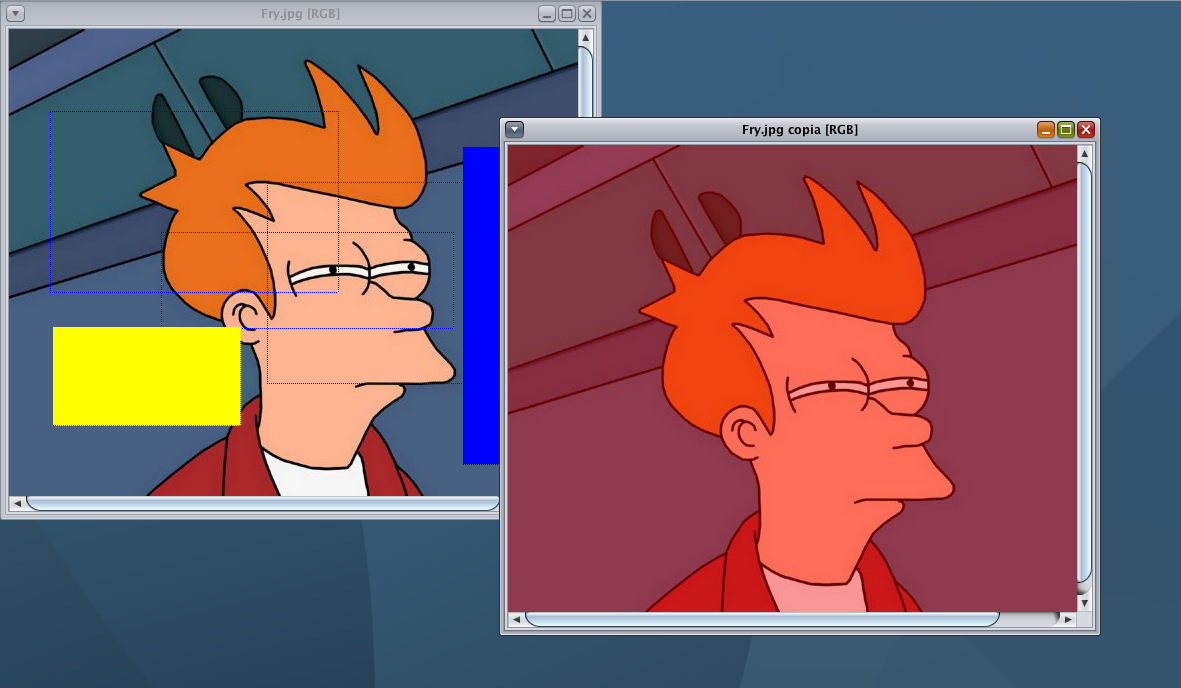
\includegraphics[width=0.5\textwidth]{imagenes/duplicar2.jpg}
 \caption{Duplicar imagen}
 \label{diseño}
 \end{figure}
\subsubsection{Modificar brillo}
\vskip0.3cm
\begin{figure}[H]
 \centering
  
\includegraphics[width=0.3\textwidth]{imagenes/fryBrilo2.jpg}
  
\includegraphics[width=0.3\textwidth]{imagenes/Fry.jpg}
  
\includegraphics[width=0.3\textwidth]{imagenes/fryBrillo1.jpg}
 \caption{Modificación del brillo}
 \label{diseño}
\end{figure}
\subsubsection{Filtro de emborronamiento}
Se ha aplicado varias veces el filtro para que sea visible.
\vskip0.3cm
\begin{figure}[H]
 \centering
  
\includegraphics[width=0.3\textwidth]{imagenes/Fry.jpg}
  
\includegraphics[width=0.3\textwidth]{imagenes/fryEmborronamiento.jpg}
 \caption{Aplicación filtro emborronamiento}
 \label{diseño}
\end{figure}
\subsubsection{Filtro de enfoque}
\vskip0.3cm
\begin{figure}[H]
 \centering
  
\includegraphics[width=0.3\textwidth]{imagenes/Fry.jpg}
  
\includegraphics[width=0.3\textwidth]{imagenes/fryEnfoque.jpg}
 \caption{Aplicación filtro enfoque}
 \label{diseño}
\end{figure}
\subsubsection{Filtro de relieve}
\vskip0.3cm
\begin{figure}[H]
 \centering
  
\includegraphics[width=0.3\textwidth]{imagenes/Fry.jpg}
  
\includegraphics[width=0.3\textwidth]{imagenes/fryRelieve.jpg}
 \caption{Aplicación filtro relieve}
 \label{diseño}
\end{figure}
\subsubsection{Contraste normal}
\vskip0.3cm
\begin{figure}[H]
 \centering
  
\includegraphics[width=0.3\textwidth]{imagenes/Fry.jpg}
  
\includegraphics[width=0.3\textwidth]{imagenes/fryContraste.jpg}
 \caption{Aplicación contraste}
 \label{diseño}
\end{figure}
\subsubsection{Iluminado}
\vskip0.3cm
\begin{figure}[H]
 \centering
  
\includegraphics[width=0.3\textwidth]{imagenes/Fry.jpg}
  
\includegraphics[width=0.3\textwidth]{imagenes/fryIluminado.jpg}
 \caption{Aplicación iluminación}
 \label{diseño}
\end{figure}
\subsubsection{Oscurecido}
\vskip0.3cm
\begin{figure}[H]
 \centering
  
\includegraphics[width=0.3\textwidth]{imagenes/Fry.jpg}
  
\includegraphics[width=0.3\textwidth]{imagenes/fryOscurecido.jpg}
 \caption{Aplicación oscurecido}
 \label{diseño}
\end{figure}
\subsubsection{Invertir colores}
\vskip0.3cm
\begin{figure}[H]
 \centering
  
\includegraphics[width=0.3\textwidth]{imagenes/Fry.jpg}
  
\includegraphics[width=0.3\textwidth]{imagenes/fryNegativo.jpg}
 \caption{Aplicación filtro negativo}
 \label{diseño}
\end{figure}
\subsubsection{Conversión a espacios RGB, YCC, GRAY}
Para comprobar que la conversión se ha realizado correctamente, se extraen las bandas de colores y se comparan. En la imagen se pueden ver la tercera banda de una imagen en espacio de color RGB y YCC, respectivamente.
\vskip0.3cm
\begin{figure}[H]
 \centering
  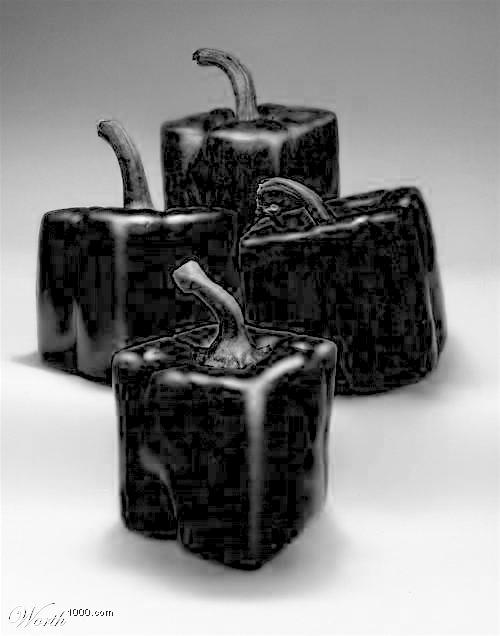
\includegraphics[width=0.3\textwidth]{imagenes/banda3RGB.jpg}
  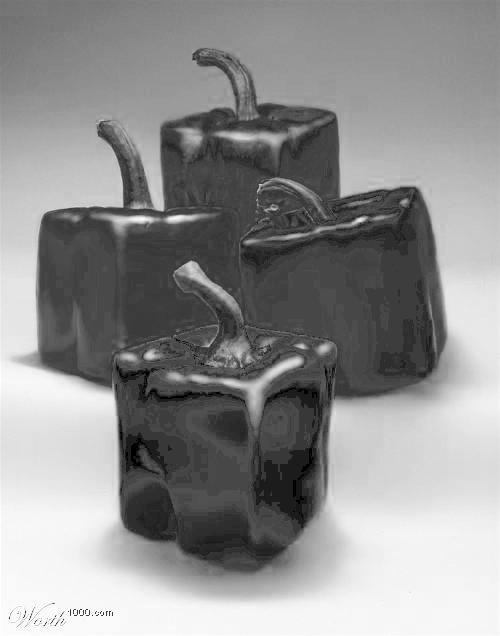
\includegraphics[width=0.3\textwidth]{imagenes/banda3YCC.jpg}
 \caption{}
 \label{diseño}
\end{figure}
\subsubsection{Giro libre}
\vskip0.3cm
\begin{figure}[H]
 \centering
  
\includegraphics[width=0.3\textwidth]{imagenes/Fry.jpg}
  
\includegraphics[width=0.3\textwidth]{imagenes/fryGiro.jpg}
 \caption{Giro libre}
 \label{diseño}
\end{figure}
\subsubsection{Escalado}
\subsubsection{Tintado}
\vskip0.3cm
\begin{figure}[H]
 \centering
  
\includegraphics[width=0.3\textwidth]{imagenes/fryTinteRojo.jpg}
  
\includegraphics[width=0.3\textwidth]{imagenes/Fry.jpg}
  
\includegraphics[width=0.3\textwidth]{imagenes/fryTinteAmarillo.jpg}
 \caption{Tintado de la imagen}
 \label{diseño}
\end{figure}
\subsubsection{Ecualización}
\vskip0.3cm
\begin{figure}[H]
 \centering
  
\includegraphics[width=0.3\textwidth]{imagenes/Fry.jpg}
  
\includegraphics[width=0.3\textwidth]{imagenes/fryEcualizacion.jpg}
 \caption{Aplicación ecualización}
 \label{diseño}
\end{figure}
\subsubsection{Filtro sepia}
\vskip0.3cm
\begin{figure}[H]
 \centering
  
\includegraphics[width=0.3\textwidth]{imagenes/Fry.jpg}
  
\includegraphics[width=0.3\textwidth]{imagenes/frySepia.jpg}
 \caption{Aplicación filtro sepia}
 \label{diseño}
\end{figure}
\subsubsection{Umbralización}
\vskip0.3cm
\begin{figure}[H]
 \centering
  
\includegraphics[width=0.3\textwidth]{imagenes/Fry.jpg}
  \includegraphics[width=0.3\textwidth]{imagenes/fryUmbralizado.jpg}
 \caption{Umbralizar imagen}
 \label{diseño}
\end{figure}
\subsubsection{Operador \textit{LookupOp} basado en una función propia}
\vskip0.3cm
\begin{figure}[H]
 \centering
  \includegraphics[width=0.3\textwidth]{imagenes/Fry.jpg}
  \includegraphics[width=0.3\textwidth]{imagenes/fryCos.jpg}
 \caption{Operación cosinusoide}
 \label{diseño}
 \end{figure}
\subsubsection{Operación de diseño propio: filtro violeta}
\vskip0.3cm
\begin{figure}[H]
 \centering
  \includegraphics[width=0.3\textwidth]{imagenes/Fry.jpg}
  \includegraphics[width=0.3\textwidth]{imagenes/fryVioleta.jpg}
 \caption{Aplicación filtro violeta}
 \label{diseño}
 \end{figure}
\subsection{Sonido}
\subsection{Vídeo}
A continuación se muestran las funcionalidades del vídeo y la cámara.
\subsubsection{WebCam}
En primer lugar, comprobamos que puede abrirse correctamente la cámara. Una vez hecho esto, se comprobará si se realizan las capturas de pantalla correctamente. Si no hay ventana de cámara abierta, no se podrá sacar ninguna captura de pantalla.
\vskip0.3cm
\begin{figure}[H]
 \centering
  \includegraphics[width=0.8\textwidth]{video/webcam.jpg}
 \caption{Webcam abierta}
 \label{diseño}
 \end{figure}
 \vskip0.3cm
\begin{figure}[H]
 \centering
  \includegraphics[width=0.8\textwidth]{video/captura.jpg}
 \caption{Captura de pantalla}
 \label{diseño}
 \end{figure}
%\section{Bonus}

%\begin{lstlisting}[language=python, caption=Código gradiente descendente, label=lst:graddesc]
%\end{lstlisting}
%\renewcommand{\labelenumi}{\alph{enumi})}

%%BIBLIOGRAFIA%%
%\clearpage
%\begin{thebibliography}{X}

%\end{thebibliography}
\end{document}
